\section*{Chapter 3: Design and Implementation}
\phantomsection \setcounter{section}{3} \setcounter{subsection}{0}
\addcontentsline{toc}{section}{\textit{Chapter 3: Design and Implementation}}

This chapter describes the dataset, preprocessing pipeline, proposed model architecture, baseline models, and experimental setup used in this study.

\subsection{University of Bonn EEG Dataset Description}

The University of Bonn EEG dataset \cite{andrzejak2001} is one of the most widely used benchmark datasets for epileptic seizure detection research. It consists of five subsets (denoted A--E, or equivalently Z, O, N, F, S), each containing 100 single-channel EEG segments of 23.6 seconds duration. All signals were sampled at 173.61~Hz with 12-bit analog-to-digital conversion, resulting in 4097 data points per recording. A hardware bandpass filter with settings of 0.53--40~Hz (12~dB/oct) was applied during acquisition, eliminating the need for additional frequency-domain filtering in preprocessing.

Table~\ref{table:bonn_dataset} summarises the five subsets and their clinical characteristics.

\begin{table}[h]
  \centering
  \begin{spacing}{1.35}
  \caption{University of Bonn EEG Dataset Description}\vspace{0.7em}
  \label{table:bonn_dataset}
    \begin{tabular}{|p{1.5cm}|p{1.5cm}|p{5.5cm}|p{3cm}|p{2cm}|}
    \hline
    \textbf{Subset} & \textbf{Label} & \textbf{Description} & \textbf{Recording Type} & \textbf{Recordings} \\
    \hline
    Z (Set A) & Normal & Healthy volunteers, eyes open & Surface EEG & 100 \\
    \hline
    O (Set B) & Normal & Healthy volunteers, eyes closed & Surface EEG & 100 \\
    \hline
    N (Set C) & Inter-ictal & Epilepsy patients, seizure-free (contralateral hemisphere) & Intracranial EEG & 100 \\
    \hline
    F (Set D) & Inter-ictal & Epilepsy patients, seizure-free (epileptogenic zone) & Intracranial EEG & 100 \\
    \hline
    S (Set E) & Ictal & Epilepsy patients, during seizure & Intracranial EEG & 100 \\
    \hline
    \end{tabular}
  \end{spacing}
\end{table}

Three classification tasks of increasing difficulty are defined to comprehensively evaluate the model:

\begin{itemize}
    \item \textbf{Binary classification}: Normal (Z+O, 200 recordings) vs.\ Seizure (S, 100 recordings).
    \item \textbf{Three-class classification}: Normal (Z+O) vs.\ Inter-ictal (N+F) vs.\ Seizure (S).
    \item \textbf{Five-class classification}: Z vs.\ O vs.\ N vs.\ F vs.\ S (the most challenging task, requiring discrimination between physiologically similar subsets).
\end{itemize}

Figure~\ref{fig:signal_comparison} illustrates representative EEG waveforms from each subset. Normal recordings (Z, O) exhibit low-amplitude signals typically within $\pm$200~$\mu$V, while seizure recordings (S) display high-amplitude, rhythmic discharges frequently exceeding $\pm$1000~$\mu$V. The inter-ictal recordings (N, F) show intermediate characteristics with occasional epileptiform discharges.

\begin{figure}[h]
\centering
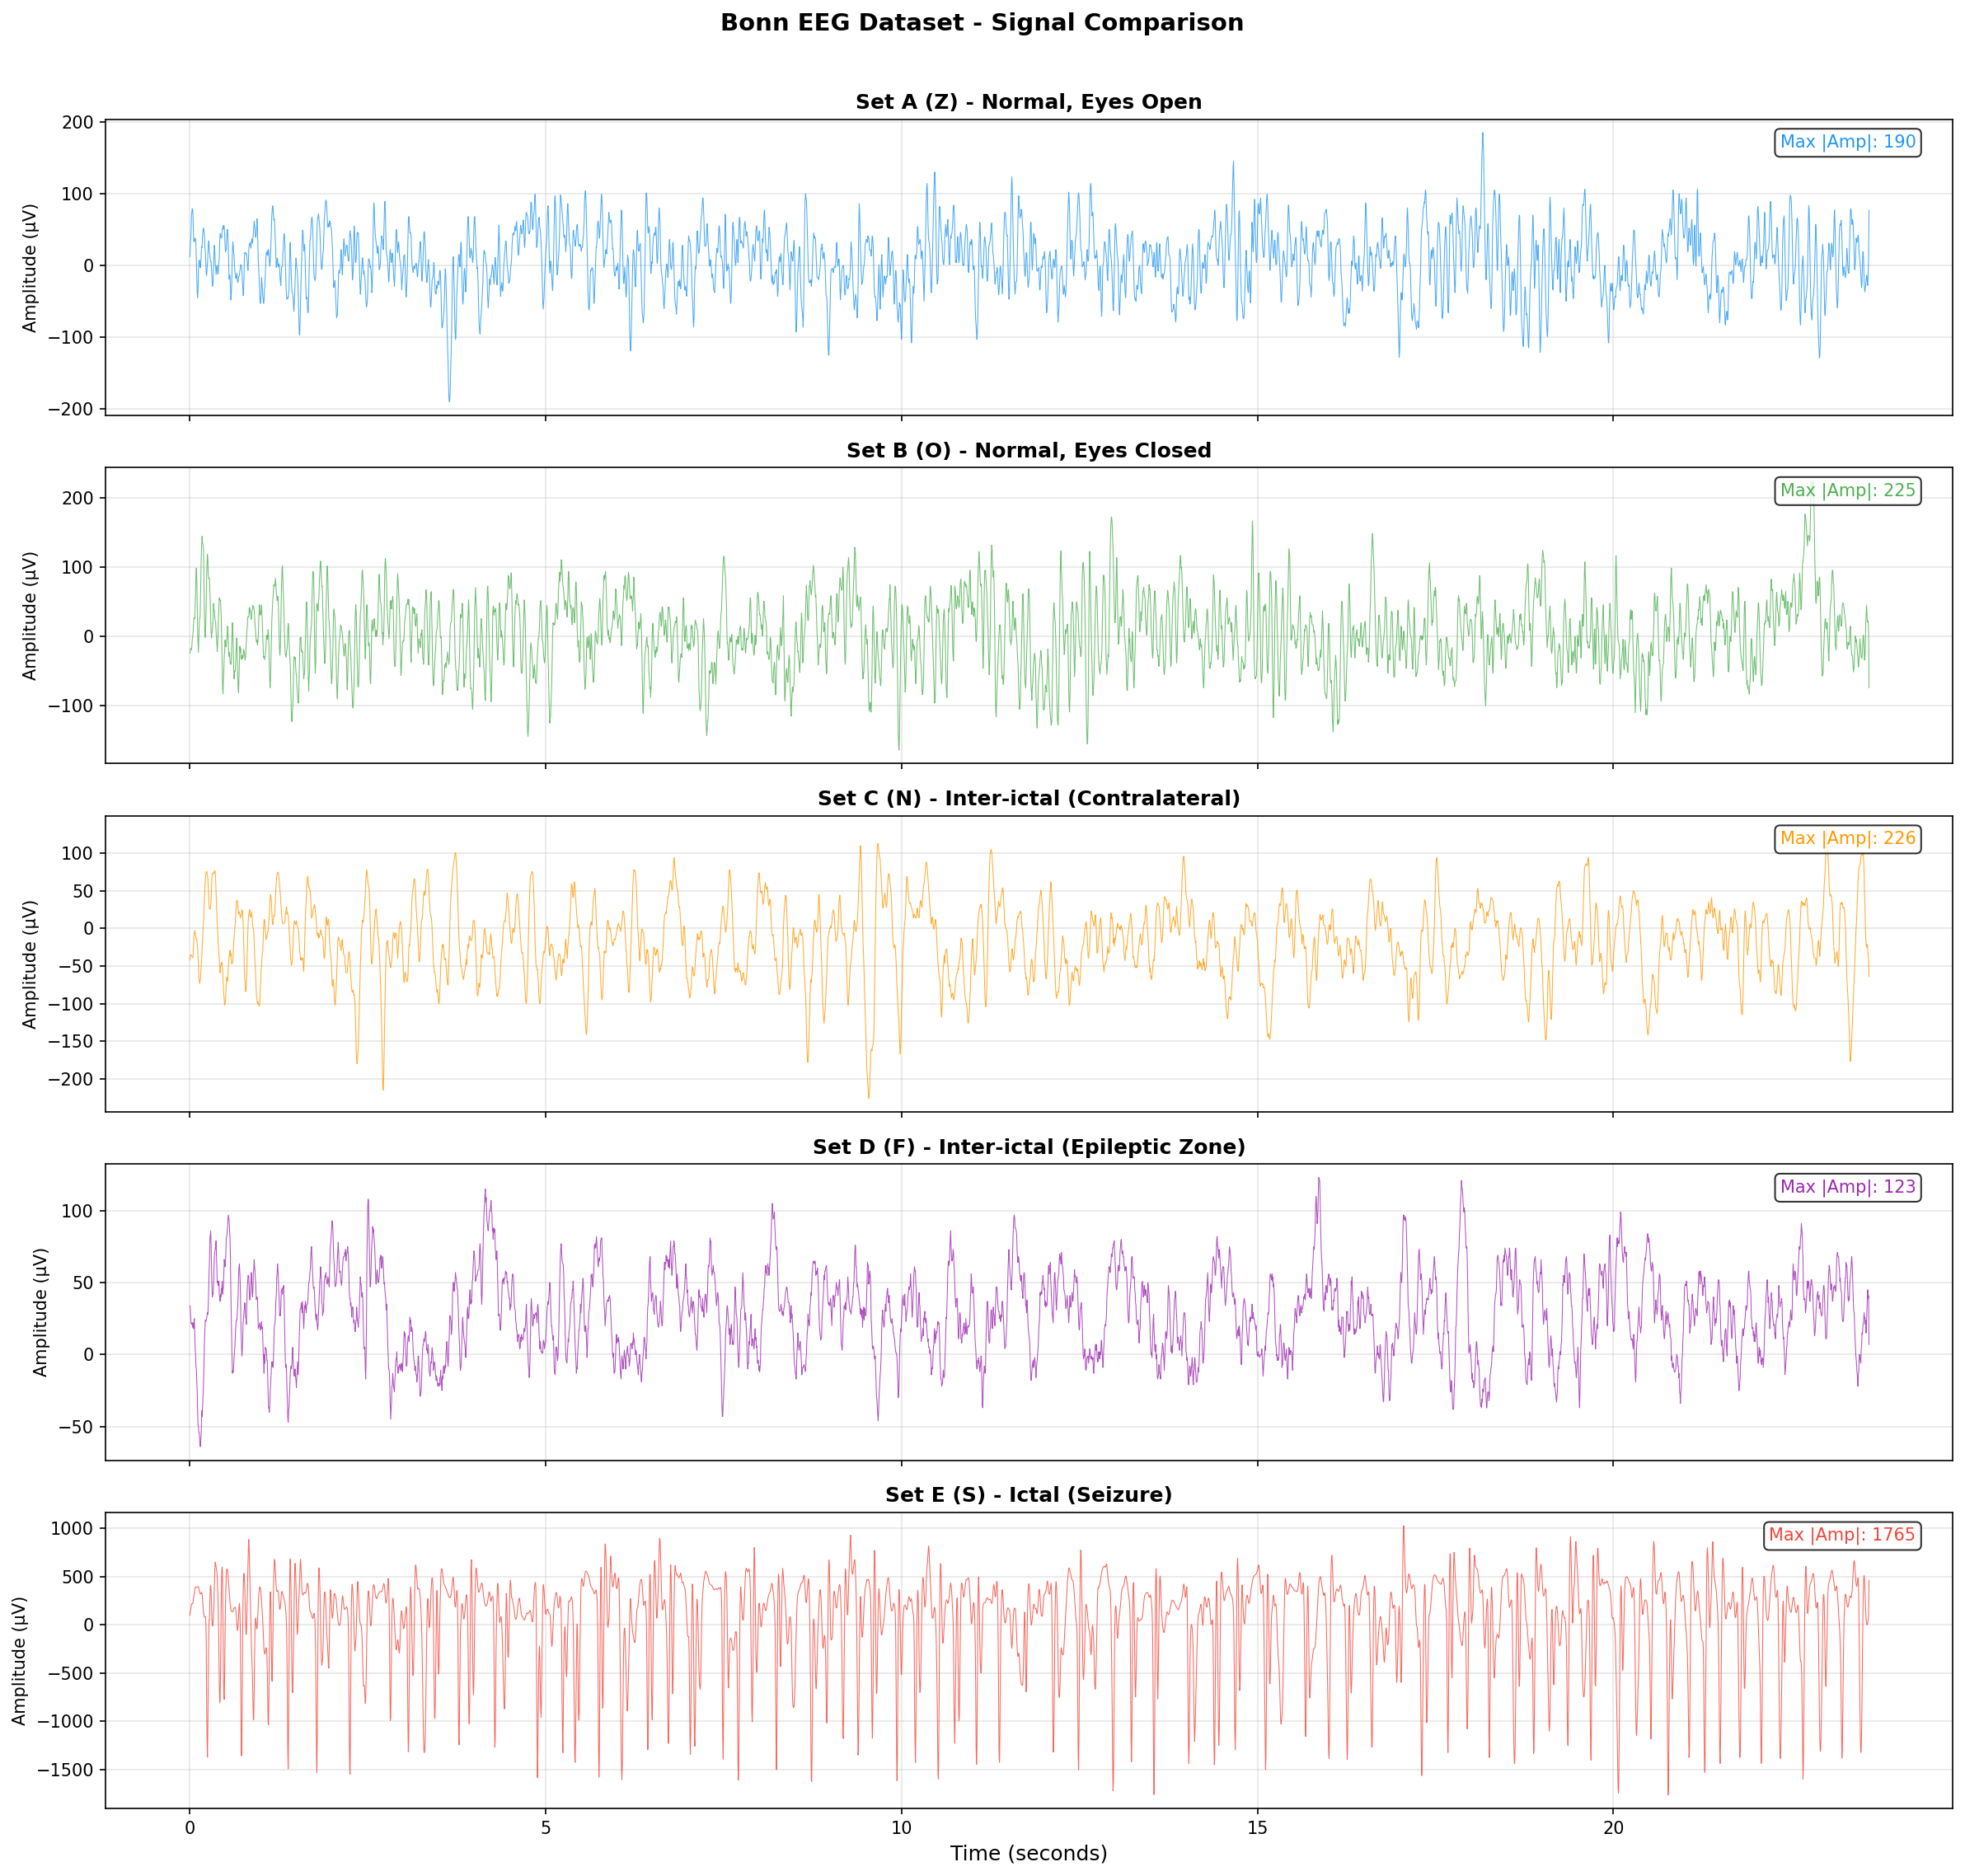
\includegraphics[width=\textwidth]{figures/signal_comparison.png}
\caption{Representative EEG signal waveforms from the five subsets of the Bonn dataset}
\label{fig:signal_comparison}
\end{figure}

\subsection{EEG Signal Preprocessing Pipeline}

The preprocessing pipeline was designed with particular emphasis on preventing data leakage, a methodological concern raised by the project supervisor and commonly overlooked in related literature.

\subsubsection{Recording-level K-Fold Cross-Validation}

A strict recording-level 10-Fold Stratified Cross-Validation strategy is employed. In each fold, the dataset is first split at the \textit{recording} level --- all sliding-window segments derived from a single original EEG recording are kept entirely within either the training or validation set, never split across both. This prevents the model from ``seeing'' overlapping segments of the same recording during both training and evaluation.

This approach differs from the segment-level splitting used by many prior studies (e.g., Thara et al. \cite{thara2019}), where individual segments are shuffled independently, allowing fragments of the same recording to appear in both training and validation sets. Such leakage inflates reported accuracy, particularly when segments overlap.

\subsubsection{Data Leakage Discovery and Correction}

An earlier version of this project's pipeline applied sliding-window segmentation \textit{before} the train/validation split, which constituted a data leakage vulnerability. Combined with a globally-fitted StandardScaler, this resulted in artificially inflated accuracy (99.95\% on binary classification). After identifying this issue, the pipeline was refactored to ensure:

\begin{enumerate}
    \item Recording-level splitting is performed \textit{first}.
    \item Sliding-window segmentation is applied \textit{independently} to training and validation recordings.
    \item The StandardScaler is fitted exclusively on training data, then applied to transform validation data.
\end{enumerate}

After correction, the binary accuracy decreased from 99.95\% to 99.67\%, and the five-class accuracy from 86.60\% to 84.51\%, confirming a more rigorous evaluation framework.

\subsubsection{Sliding Window Segmentation}

Each 4097-point recording is segmented using a sliding window of 1024 data points ($\approx$5.9 seconds at 173.61~Hz) with 50\% overlap (stride = 512 points). This produces approximately 7 segments per recording and expands the effective dataset from 500 original recordings to approximately 3{,}500 training samples, mitigating the risk of overfitting on the small raw dataset.

\subsubsection{Z-Score Normalisation}

A global Z-Score normalisation is applied using \texttt{StandardScaler}: a single mean and standard deviation are computed across all data points in the training set of each fold, then used to transform both training and validation data. This approach preserves inter-window amplitude differences --- an important discriminative feature, as seizure signals exhibit significantly higher amplitudes than normal recordings.

\subsection{Proposed Hybrid Model Architecture}

The proposed model is a hybrid deep learning architecture combining three complementary components: a 1D Convolutional Neural Network (1D-CNN) for local feature extraction, a Bidirectional Long Short-Term Memory network (Bi-LSTM) for temporal dependency modelling, and a Self-Attention mechanism for focusing on discriminative time steps. Table~\ref{table:model_architecture} summarises the architecture.

\begin{table}[h]
  \centering
  \begin{spacing}{1.35}
  \caption{Proposed Hybrid Model Architecture}\vspace{0.7em}
  \label{table:model_architecture}
    \begin{tabular}{|p{2.5cm}|p{7cm}|p{4cm}|}
    \hline
    \textbf{Component} & \textbf{Configuration} & \textbf{Role} \\
    \hline
    1D-CNN Layer~1 & Conv1D(1$\rightarrow$64, kernel=7), BN, ReLU, MaxPool(2), Dropout(0.2) & Local feature extraction \\
    \hline
    1D-CNN Layer~2 & Conv1D(64$\rightarrow$128, kernel=7), BN, ReLU, MaxPool(2), Dropout(0.2) & Higher-level local patterns \\
    \hline
    Bi-LSTM Layer~1 & 128 hidden units, bidirectional, Dropout(0.4) & Forward/backward temporal modelling \\
    \hline
    Bi-LSTM Layer~2 & 64 hidden units, bidirectional, Dropout(0.4) & Refined temporal representation \\
    \hline
    Self-Attention & 64-dim, tanh scoring, softmax weighting & Focus on key time steps \\
    \hline
    Classifier & Dense(128$\rightarrow$64), ReLU, Dropout(0.4), Output & Classification head \\
    \hline
    \end{tabular}
  \end{spacing}
\end{table}

\subsubsection{1D-CNN Feature Extraction}

The 1D-CNN module consists of two convolutional layers with 64 and 128 filters respectively, each with a kernel size of 7. Each layer is followed by Batch Normalisation, ReLU activation, max-pooling (factor 2), and dropout (rate 0.2). The CNN extracts local spatio-temporal features such as spike-wave complexes and sharp transients that are characteristic of epileptic activity. The two max-pooling operations reduce the temporal resolution by a factor of 4, compressing the 1024-point input to a 256-step feature sequence.

\subsubsection{Bidirectional LSTM}

The output of the CNN is passed to two stacked Bi-LSTM layers with 128 and 64 hidden units respectively. Each Bi-LSTM processes the sequence in both forward and backward directions, producing output vectors of dimension $2 \times \text{hidden\_units}$ at each time step. This bidirectional processing captures both past and future temporal context, which is essential for modelling the evolution of seizure dynamics over time.

\subsubsection{Self-Attention Mechanism}

The Self-Attention layer computes an importance weight $\alpha_t$ for each time step $t$ of the Bi-LSTM output $h_t$:
\begin{equation}
e_t = \tanh(\mathbf{W} h_t + b)
\end{equation}
\begin{equation}
\alpha_t = \frac{\exp(\mathbf{u}^\top e_t)}{\sum_{j=1}^{T} \exp(\mathbf{u}^\top e_j)}
\end{equation}
\begin{equation}
c = \sum_{t=1}^{T} \alpha_t h_t
\end{equation}
where $\mathbf{W} \in \mathbb{R}^{128 \times 64}$ and $\mathbf{u} \in \mathbb{R}^{64}$ are learnable parameters. The context vector $c$ is a weighted sum of all time steps, allowing the model to focus on the most discriminative temporal regions rather than treating all time steps equally.

\subsubsection{Output Layer}

For binary classification, the output layer consists of a single neuron with sigmoid activation, trained with Binary Cross-Entropy with Logits Loss. For three-class and five-class tasks, the output layer has $N$ neurons (where $N$ is the number of classes) with softmax activation (implicitly applied through Cross-Entropy Loss). The total number of trainable parameters is approximately 504{,}000 (1.92~MB).

\subsection{Baseline Models for Comparative Analysis}

Three baseline models were implemented to serve as an ablation study, systematically evaluating the contribution of each component in the hybrid architecture. Table~\ref{table:baselines} summarises the baselines and their roles.

\begin{table}[h]
  \centering
  \begin{spacing}{1.35}
  \caption{Baseline Models for Ablation Study}\vspace{0.7em}
  \label{table:baselines}
    \begin{tabular}{|p{2.8cm}|p{6.2cm}|p{4.5cm}|}
    \hline
    \textbf{Baseline} & \textbf{Architecture} & \textbf{Ablation Purpose} \\
    \hline
    SVM + Wavelet Packet & RBF-SVM on 64-dim WPD features (Daubechies-4, 4 levels) & Traditional ML reference \\
    \hline
    Pure 1D-CNN & 4-layer CNN (32$\rightarrow$64$\rightarrow$128$\rightarrow$128) + Global Average Pooling & Remove temporal modelling \\
    \hline
    Pure Bi-LSTM + Attention & 2-layer Bi-LSTM (128, 64) + Self-Attention (no CNN) & Remove local feature extraction (no CNN) \\
    \hline
    \end{tabular}
  \end{spacing}
\end{table}

The SVM baseline uses Wavelet Packet Decomposition to extract 16 sub-band nodes, from which four statistical features (energy, mean, standard deviation, and Shannon entropy) are computed per node, yielding a 64-dimensional feature vector per recording. A Radial Basis Function (RBF) kernel SVM is then trained on these features. Notably, the SVM operates on complete recordings without sliding-window segmentation, making its K-Fold split inherently at the recording level.

\subsection{Experimental Setup and Training Strategy}

Table~\ref{table:training_config} lists the training hyperparameters used for all deep learning models.

\begin{table}[h]
  \centering
  \begin{spacing}{1.35}
  \caption{Training Hyperparameters}\vspace{0.7em}
  \label{table:training_config}
    \begin{tabular}{|p{5cm}|p{5cm}|}
    \hline
    \textbf{Parameter} & \textbf{Value} \\
    \hline
    Optimiser & Adam \\
    \hline
    Learning rate & $1 \times 10^{-4}$ \\
    \hline
    LR scheduler & ReduceLROnPlateau (factor=0.5, patience=7) \\
    \hline
    Early stopping patience & 15 epochs \\
    \hline
    Maximum epochs & 100 \\
    \hline
    Batch size & 64 \\
    \hline
    Cross-validation & 10-Fold Stratified, recording-level \\
    \hline
    Random seed & 42 \\
    \hline
    \end{tabular}
  \end{spacing}
\end{table}

All deep learning experiments were conducted on an NVIDIA GeForce RTX 3070 Ti GPU (8~GB VRAM) using PyTorch 2.x with CUDA acceleration. The framework was migrated from TensorFlow/Keras due to the discontinuation of native Windows GPU support in TensorFlow 2.11 and later versions, which resulted in an approximately 80$\times$ speedup (from $\sim$55~s to $\sim$0.7~s per training epoch).

The evaluation metrics used throughout this study are:
\begin{itemize}
    \item \textbf{Accuracy}: The proportion of correctly classified samples.
    \item \textbf{Weighted F1 Score}: The harmonic mean of precision and recall, weighted by class support, to account for potential class imbalance.
    \item \textbf{Confusion Matrix}: Visualisation of per-class classification performance.
    \item \textbf{Paired t-test}: Statistical significance testing across cross-validation folds to determine whether observed performance differences are statistically reliable ($p < 0.05$).
\end{itemize}
